\subsection{Login}

All'avvio il sito presenta una schermata di accesso, in cui gli utenti sono invitati a inserire le proprie credenziali (username e password) per ottenere l'accesso al sistema. Si precisa che solo gli utenti autorizzati hanno il permesso di accedere al servizio. Dopo aver compilato correttamente i campi richiesti, l'utente può procedere cliccando sul pulsante di Login, il quale lo reindirizzerà alla dashboard principale del sistema.\\
\begin{figure}[H]
    \centering
    \fbox{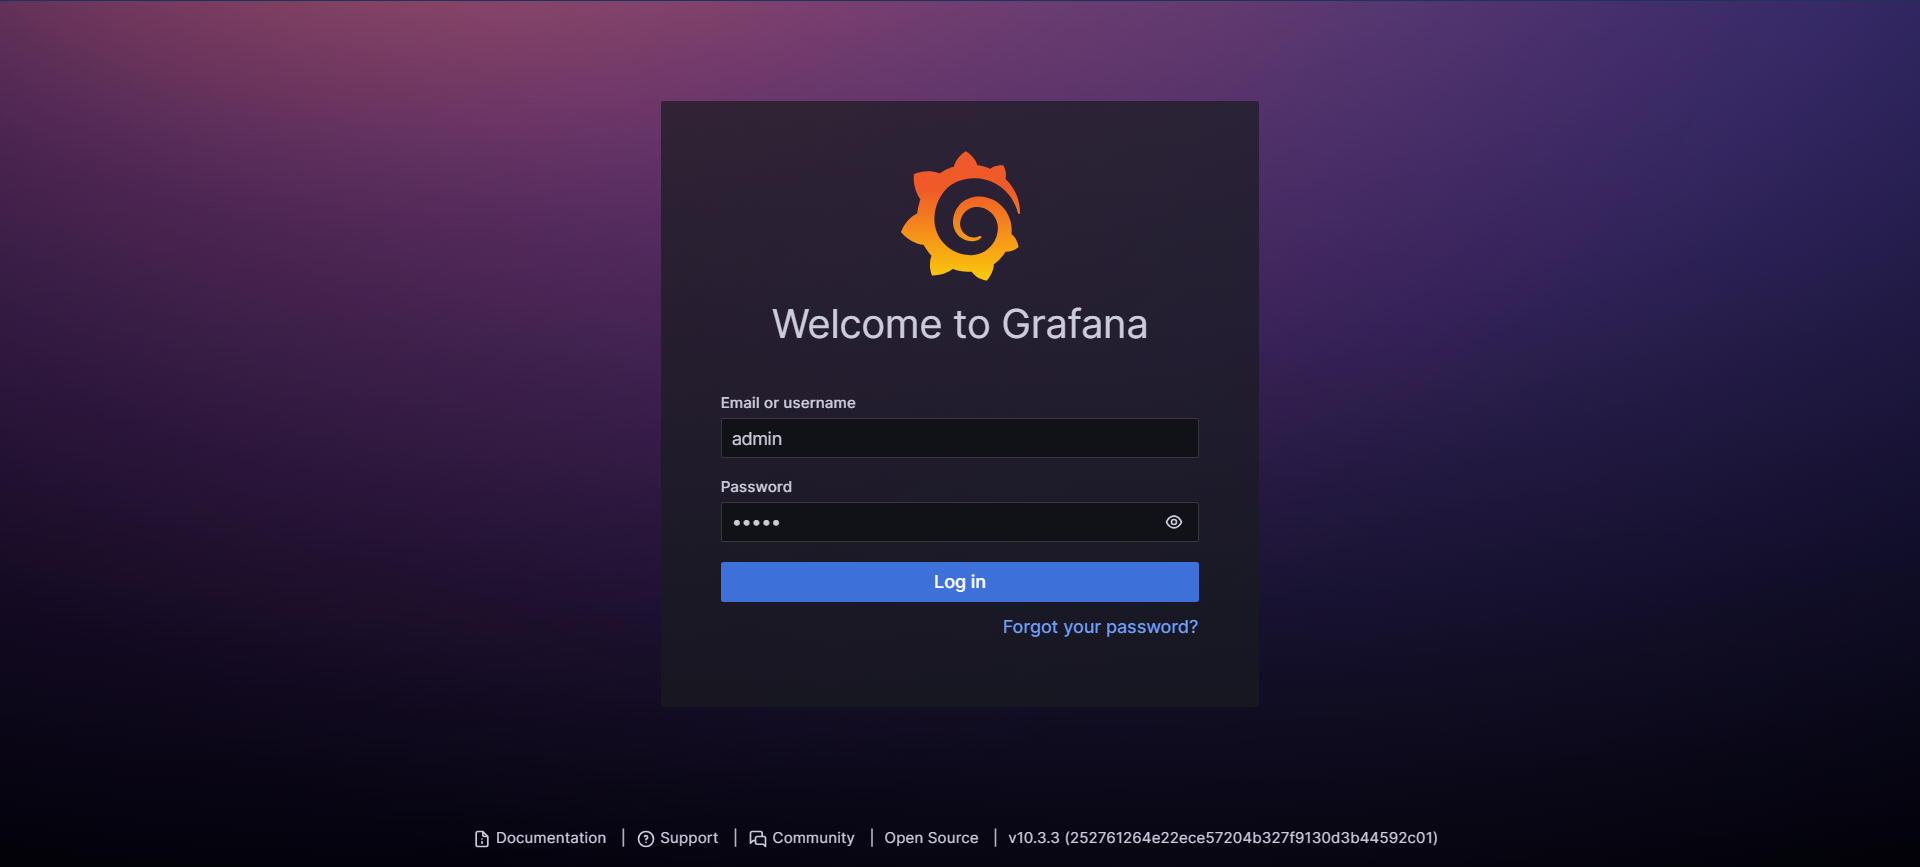
\includegraphics[width=13cm]{../Images/ManualeUtente/login.png}}
    \caption{Schermata di accesso al sistema}
    \label{fig:my_label}
\end{figure}
Nel caso in cui le credenziali siano errate, il sistema mostrerà un messaggio di errore all’utente:\\
\begin{figure}[H]
    \centering
    \fbox{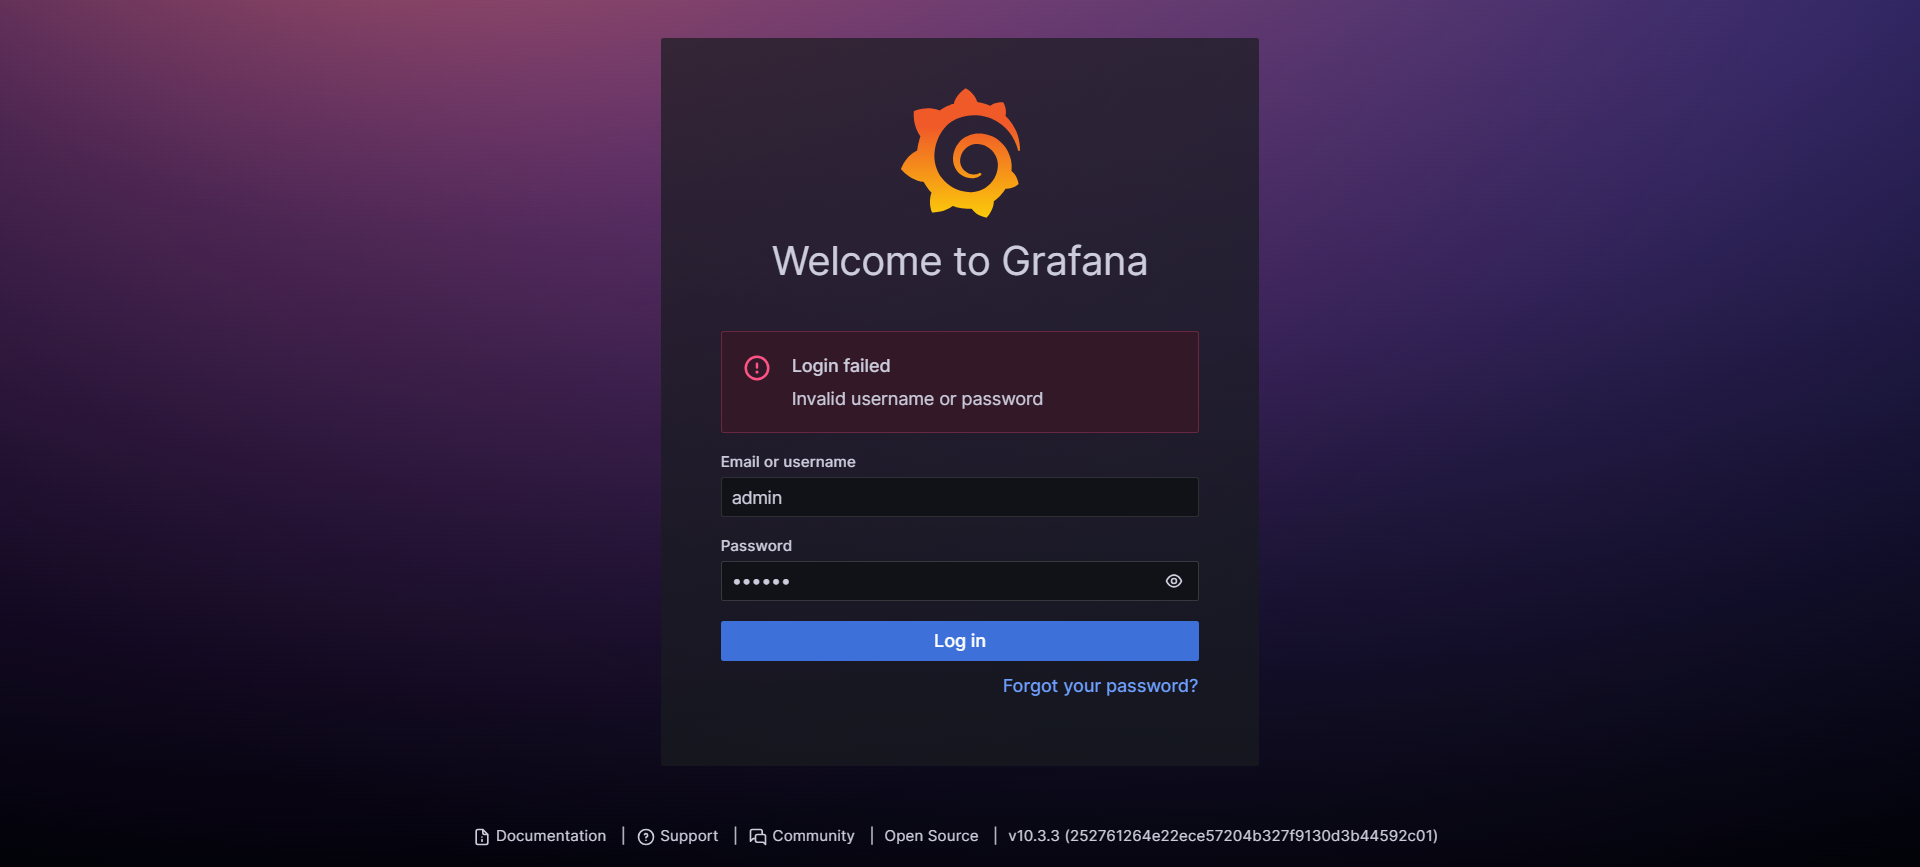
\includegraphics[width=13cm]{../Images/ManualeUtente/login-error-username_wide.png}}
    \caption{Messaggio di errore per username errato}
    \label{fig:my_label}
\end{figure}